\documentclass[a4paper,12pt,oneside,openany,xelatex,ja=standard,jafont=noto]{bxjsbook}
%
\usepackage{amsmath,amssymb}
\usepackage{graphicx}
\usepackage{url}
\usepackage{booktabs}
\usepackage{multirow}
\usepackage{klisb} % 卒業論文フォーマット
%
\title{文脈誘導型ランキング学習}
%\subtitle{サブタイトル} % 基本的に利用しない
\studentid{123456789} % 学生番号
\author{加藤 誠} % 自分の氏名.姓名の間は全角スペース
\affiliation{筑波大学 情報学群\\知識情報・図書館学類}
\gradyear{2021} % 基本的に卒業論文の翌年となるので注意
\gradmonth{3} % 基本的に3月か9月
\supervisor{加藤 誠}
%
\begin{document}
% 「TC:ignore」から「TC:endignore」までは文字カウントが無視される
%TC:ignore
%
\maketitle
%
\frontmatter
%
% 抄録
\begin{abst}
本論文では,順序付けられた一部のエンティティを訓練データ,エンティティの数値属性を特徴として線形関数を学習することで,エンティティのランキングを行う問題に取り組む.
例えば,$f($Entity$) = +0.5($GDP$) − 0.8($自殺者数$)$という関数を「幸福度」によって順序づけられたエンティティから学習する.
この問題では訓練データの数が非常に少ないため,
Web上に存在する大量の「文脈」による補助を受けて学習を行う機械学習手法,
文脈誘導型学習を本論文では提案する.
実験では3クラスのエンティティについて158個の様々な順序によるランキングを行った.
実験結果から,既存のランキング学習手法よりも高い精度が文脈誘導型学習によって得られることが明らかとなった.
本論文では,順序付けられた一部のエンティティを訓練データ,エンティティの数値属性を特徴として線形関数を学習することで,エンティティのランキングを行う問題に取り組む.
例えば,$f($Entity$) = +0.5($GDP$) − 0.8($自殺者数$)$という関数を「幸福度」によって順序づけられたエンティティから学習する.
この問題では訓練データの数が非常に少ないため,
Web上に存在する大量の「文脈」による補助を受けて学習を行う機械学習手法,
文脈誘導型学習を本論文では提案する.
実験では3クラスのエンティティについて158個の様々な順序によるランキングを行った.
実験結果から,既存のランキング学習手法よりも高い精度が文脈誘導型学習によって得られることが明らかとなった.
本論文では,順序付けられた一部のエンティティを訓練データ,エンティティの数値属性を特徴として線形関数を学習することで,エンティティのランキングを行う問題に取り組む.
例えば,$f($Entity$) = +0.5($GDP$) − 0.8($自殺者数$)$という関数を「幸福度」によって順序づけられたエンティティから学習する.
この問題では訓練データの数が非常に少ないため,
Web上に存在する大量の「文脈」による補助を受けて学習を行う機械学習手法,
文脈誘導型学習を本論文では提案する.
実験では3クラスのエンティティについて158個の様々な順序によるランキングを行った.実験結果から,既存のランキング学習手法よりも高い精度が文脈誘導型学習によって得られることが明らかとなった.
実験では3クラスのエンティティについて158個の様々な順序によるランキングを行った.実験結果から,既存のランキング学習手法よりも高い精度が文脈誘導型学習によって得られることが明らかとなった.
実験では3クラスのエンティティについて158個の様々な順序によるランキングを行った.実験結果から,既存のランキング学習手法よりも高い精度が文脈誘導型学習によって得られることが明らかとなった.
実験では3クラスのエンティティについて158個の様々な順序によるランキングを行った.

\end{abst}
%
\setcounter{tocdepth}{3}
\tableofcontents
\thispagestyle{empty}
%
\mainmatter
%TC:endignore
%
% 本文
\chapter{序論}
\label{sq:Introduction}
エンティティの順序は人気の高いコンテンツであり,多くのWebサイトで紹介されている.
例えば,国,都市,企業,有名人,および,製品などが,居住性,革新性,美しさ,性能などのさまざまな基準によって順序づけられている.
順序は比較文
(例えば, ``レオナルド ディカプリオはブラッド ピットよりも背が高い'')や,
最上級(例えば,``東京は最も物価の高い都市である''),
ランキング(例えば,``1位:デンマーク,2位:スイス,3位:アイスランド'')などの形式で表現されている.
人々はそのようなエンティティの順序を意思決定,比較,計画などに利用する.

順序づけの基準の詳細は,場合によっては正確かつ客観的に記述されているが,
省略されたり基準が主観的である場合もある.
例えば,デンマークはいくつかのウェブサイトで最も幸せな国として紹介されているが詳細な証拠が提示されていない場合も多い.
その根拠は,国民の自己申告,他の国の評判,あるいは,
GDPや自殺者数などの客観的尺度かもしれない.
不確かな証拠だけでそのような知識を獲得することは,
偏見やステレオタイプにつながる可能性がある.

本論文では,部分的に観測された順序を訓練データとして,エンティティの数値属性を特徴として使用することで,エンティティの順序を学習する方法を提案する.
学習されたモデルによって,Web上の順序を説明することが可能であり,
また,学習に使用されていない他のエンティティをランキングすることも可能である.
順序付けは数値属性の線形関数$f$によって表すことができると仮定する.
これは,主にユーザへの説明能力が高く,
現実世界における順序の大部分は,いくつかの尺度を線形結合することによって求められるという事実があるためである.
例えば,「幸福度」という「順序基準」によって順序づけられた(デンマーク,スイス,アイスランド)というエンティティ列と
「GDP」,「国土面積」,「自殺者数」という数値属性が与えられた時,
$f($Entity$) = +0.5($GDP$) − 0.8($自殺者数$)$という線形関数を学習することができる.

この問題の主な課題の1つは,訓練データが不足していることである.
多くのWebサイトでは,すべてのエンティティの順序は記述されてはいない.
さらに,一部のエンティティクラスでは,すべてのエンティティの順序が記述されていたとしても訓練データのサイズは十分ではない(たとえば,日本の都道府県数は47であり,アメリカの州の数は50である).
数値属性の数は,通常,Web上で順序づけられたエンティティの数よりもはるかに多いので,エンティティの順序を学習する際に,深刻な過学習の問題が起こりうる.

この本質的な問題に対処するために,我々は{\bf 文脈誘導型学習}と呼ばれる学習方法を提案する.
文脈誘導型学習は,順序づけられたエンティティだけでなく,
各特徴の重みを学習するために順序基準と属性に関する文脈を利用する.
文脈は追加の情報をモデルに与え,過学習を防止して学習を正しい方向に誘導する.
例えば, ``幸福度''という基準に関する線形関数の, ``GDP''という特徴に対する重みは,
(デンマーク,スイス,アイスランド)というエンティティ列だけでなく,
 ``{\bf GDP}は{\bf 幸福}のための重要な要素である''や``{\bf GDP}が向上すれば{\bf 幸福度}も改善する'',といった「幸福」と「GDP」の文脈(「幸福」と「GDP」の関係について記述された文や文書)によっても推測されることになる.
文脈誘導型学習は,文脈に対するアノテーションを必要とせず, 
代わりに,文脈と関数$f$中の重みの関係を学習するために,複数の順序を同時に学習する.
 
我々の知る限りにおいて,
文脈誘導型学習は,機械学習において「ラベル基準」と特徴の文脈を直接活用する最初の試みである(ラベル基準とはラベル付けの基準を表すテキストのことであり,エンティティランキングの問題における順序基準に対応する).
文脈誘導型学習は,ラベル基準と特徴の関係が特定のコーパスに記述されてれば,
順位付けだけでなく分類や回帰の問題にも適用することが可能である.

実験では,国,都道府県,カメラの3つのエンティティクラスを対象とし158種類の順序を学習した.
訓練された順序の精度を測定し,
与えられた順序が学習されたモデルによってどれだけ説明可能であるかを評価した.
実験の結果,文脈誘導型学習は既存のランキング学習手法よりも統計的有意に高い精度を示した.

この論文における我々の貢献を以下に示す:
(1) 数値属性を特徴とした,エンティティの順位付けを学習する問題を提案した.
これによって,Web上の順序を正確に理解し,さまざまな基準でエンティティを順序付けすることが可能である.
(2)文脈誘導型学習を提案した.これは,過学習を防止するためにラベル基準および特徴の文脈を利用する一般的な機械学習モデルである.
(3)幅広い順序に対する実験を行い,
エンティティの順序づけタスクにおいて文脈誘導型学習の有効性を示した.

本論文の構成は以下の通りである.
2節ではエンティティのランキングに関する関連研究,および,
文脈誘導型学習と他の機械学習手法との関係について述べる.
3節では問題設定を説明し,文脈誘導型学習,および.
その主問題への適用方法について述べる.
4節では実験結果を示す.
最後に,5節では今後の課題と共に本論文の結論を述べる.
\chapter{関連研究}
\label{sq:RelatedWork}
本節では,エンティティのランキングに関する関連研究,および,
文脈誘導型学習と他の機械学習手法,特にマルチタスク学習との関係について述べる.

\section{エンティティランキング}
エンティティランキングはINEXやTRECのいくつかのトラックで取り組まれてきている.
INEXのEntity Rankingトラックでは,エンティティランキングとエンティティリスト補完の2つのタスクが提案された~\cite{de2007overview,demartini2008overview,demartini2009overview}.
エンティティランキングタスクは,与えられたクエリに対して適合するエンティティを発見するタスクであり,他方,エンティティリスト補完タスクでは与えられたエンティティ例に関連するエンティティを発見するタスクであった.
TRECのエンティティトラックでは,あるエンティティ例と発見対象のエンティティタイプ,それらの関係性が与えられたときに関連するエンティティを取得する,関連エンティティ発見タスクが提案された~\cite{balog2009overview,balog2010overview,balog2011overview}.
これらのタスクでは,発見されたエンティティが与えられたエンティティ例との関連性に基づいて順序づけされることだけが求められ,関連エンティティに対して様々な順序付けを行うことまでは求められていない.

エンティティリスト補完タスクと関連エンティティ発見タスクとは別に,
エンティティのランキング学習に関する関連研究も存在する.
Kangらは与えられたクエリに関連するエンティティを発見するために,決定木ブースティングに基づくランキングアルゴリズムを用いている~\cite{kang2015learning}.
Tranらはイベントのタイムライン要約のために主要度と情報量に基づいてエンティティをランキングする手法を提案している~\cite{tran2015balancing}.
Zhouらは与えられたエンティティと特定の関係にあるようなエンティティを発見する問題に取り組んでいる~\cite{zhou2013learning}.
例えば,ユーザは``FounderOf''という関係と``Microsoft''というエンティティを入力し``Bill Gates''を得ることができる.
彼らはあるエンティティ対の関係に関する検索スニペットから得られた特徴を用いて,
訓練クエリとラベル付けされたエンティティを元に各関係についてランキングを学習した.
この研究と我々の研究は共に文脈(または検索スニペット)を用いてランキング学習を行うという点では類似するが,
我々のモデルは主にエンティティの属性に基づくものであり,エンティティ対の文脈は用いていない.

我々のタスクに類似した自然言語処理タスクもいくつか提案されている.
Iwanariらは,与えられた形容詞に基づいてエンティティを順序づける問題に取り組んでいる~\cite{iwanari2016ordering}.
手法はテキストから得られたいくつかの根拠に基づいており,
エンティティと形容詞の共起やエンティティと形容詞の依存関係,直喩,比較文などが用いられている.
このタスクには既存のランキング学習および回帰モデルが用いられている.
ある順序基準に基づいてエンティティをランキングを行うという点でこのタスクは我々のタスクと類似する.
彼らの手法は順序基準とエンティティの文脈を利用するが,
我々の手法では順序基準とエンティティの「属性」の文脈を利用している.
また,本論文ではこのタスクについて効果的な学習手法についても提案を行っている.
エンティティの数値的な属性を抽出する研究も存在するが,
我々のタスクでの順序基準は多くの場合に定量化することが困難であり,
これらの研究で提案される手法では推定できないと思われる~\cite{takamura2015estimating,davidov2010extraction,madaan2016numerical}.

\section{マルチタスク学習}

文脈誘導型学習の重要な特徴を以下に要約する:
(1) 関数$f$の重みはラベルだけでなく,ラベル基準と特徴の文脈に基づいて学習される,また,
(2) 文脈と関数$f$中の重みの関係を学習するために,複数の関数が同時に学習される.
以下では,いくつかの機械学習手法について述べ文脈誘導型学習との関連について議論する.

マルチタスク学習とは複数のタスクを同時に学習することによって個々のタスクの学習を改善する方法である~\cite{caruana1997multitask}.
文脈誘導型学習はマルチタスク学習の一種であると考えられる.
EvgeniouとPontilによって提案された正則化マルチタスク学習は
複数のタスクにおける関数の重みが似ていることを仮定している~\cite{evgeniou2004regularized}.
後に述べるように,彼らのモデルは我々のモデルの特殊な場合であり,
すべての文脈が同じである場合に等価なモデルとなる.
また,共通の事前分布から重みが生成されることを仮定するモデルもある~\cite{yu2005learning,lee2007learning,daume2009bayesian}.
Argyriouらは重みが複数のタスクに共通する低次の部分空間において表現できることを仮定している~\cite{argyriou2008convex}.
これらのように全てのタスクが関連すると仮定する研究とは対照的に,
いくつかの研究ではどのタスクが関連し,似た重みを共有すべきか選択するようなモデルを提案している~\cite{jacob2009clustered,kumar2012learning}.
同様に,文脈誘導型学習はタスク間の類似性を文脈を用いることで暗に推定し,
似たようなタスクに対して似たような重みを推定する傾向にある.
文脈誘導型学習と他のマルチタスク学習手法の興味深い違いは,
いずれのタスクも類似しない場合においても文脈誘導型学習は適用可能であるという点である.
文脈誘導型学習は複数のタスク間でいくつかの文脈が類似することだけを仮定する.
したがって,文脈誘導型学習の適用範囲は既存のマルチタスク学習が対象とする問題に限らない.
%PanとYangが述べたように,
%マルチタスク学習の手法は転移学習用に簡単に修正することができるため(彼らのサーベイ論文の3.3節を参照~\cite{pan2010survey}),
%文脈誘導型学習は転移学習のための手法であるとも考えることができる.


最後に,文脈誘導型学習(Context-guided Learning,CGL)と似た名前を持つ機械学習手法との差違を明確にする.
文脈依存型学習(Context-{\it sensitive} Learning)はしばしば特徴の文脈(例えば,ピクセルを特徴とする場合の周辺ピクセル~\cite{bovolo2006novel}や単語を特徴とする場合の共起単語~\cite{cohen1999context}など)を用いる手法を指す.
他の場合,与えられたデータに対して選択的にモデルを用いる機械学習手法~\cite{qi2002context}や
直前・直後のデータを予測に用いる手法~\cite{metallinou2012context}を文脈依存型学習と呼ぶ.
これらの手法は主に文脈を追加の特徴として用いることに焦点を当てており,
文脈誘導型学習はモデルを変えることなく,文脈を用いてモデルの学習を改善する手法である.
さらに,文脈誘導型学習で用いられる文脈は特徴に関するものではなく,
ラベル基準と特徴に関するものである.
\chapter{提案手法}
\label{sq:Methodology}

本節では,まず部分的に観測されたエンティティの順序から,エンティティの順序を数値属性に基づいて学習する問題について説明を行う.
それから,文脈誘導型学習を導入し,その主問題への適用について述べる.

\section{問題設定}

$E$をあるクラスのエンティティ集合とし,
エンティティ順序$\preceq_{k}$を$E$上の全順序として定義する.
各順序は順序の基準を示す順序基準$l_k$を持つ.
例えば,順序基準として「住みやすさ」,「革新性」,「美しさ」,「性能」などが挙げられる.
順序付き集合$O_{\preceq_{k}}$ ($\subset E \times E$)は$e_i \preceq_{k} e_j$を満たす全てのエンティティ対の集合$(e_i, e_j) \in E \times E$である.
Web上においてエンティティ順序はこれら順序付き集合の部分集合によって表現されることが多い.
従って,エンティティ順序の学習のために観測・利用可能なのは$O'_{\preceq_{k}} \subset O_{\preceq_{k}}$である.
例えば, ``レオナルド ディカプリオはブラッド ピットよりも背が高い''という文は
$O'_{\preceq_{k}} = \{($``ブラッド ピット'', ``レオナルド ディカプリオ''$)\}$
を示し,``1位:デンマーク,2位:スイス,3位:アイスランド''というランキングは
$O'_{\preceq_{k}} = \{($``スイス'', ``デンマーク''$)$,
$($``アイスランド'', ``デンマーク''$)$, $($``アイスランド'', ``スイス''$)\}$
を示す.

我々の主目的は,各エンティティ$\preceq_{k}$に対して順序部分的に観測された順序付き集合$O'_{\preceq_{k}}$から線形関数$f_k(e_i) = {\mathbf w}_{k}^T {\mathbf e}_i$を学習することである.ただし,${\mathbf e}_i$はエンティティ$e_i \in E$の数値属性を表す$M$次元ベクトルであり,このベクトルの$d$次元目はエンティティの$a_d$という属性を表す.
我々はこの関数$f_k$がエンティティ順序$\preceq_{k}$を{\bf 保つ}ことを期待する:
つまり,任意の$e_i, e_j \in E$に対して$e_i \preceq_{k} e_j \Rightarrow f_k(e_i) \leq f_k(e_j)$を満たすことを期待する.
学習された関数$f_k$を用いることで順序基準$l_k$によってエンティティを順位付けすることが可能であり,学習された関数中において0でない重みを持つ数値属性によって順序基準を説明することができる.

先に述べたように,この問題の主となる課題は訓練データの不足である.
より正確には,数値属性の数$M$と比較して$|O'_{\preceq_{k}}|$がしばしば小さいことである.
例えば,我々の実験において「国」では$M=83$,「都道府県」では$M=137$である.
10件以下のエンティティしかランキングされていない場合,訓練データとして我々が得られるのは高々45個のエンティティペアであり,これらのクラスにおいては学習に十分な量であるとは考えにくい.
さらに,幅広い順序を扱うためには$M$はできるだけ大きい方が良い.
したがって,訓練データの不足から起こりうる過学習を防ぐためになんらかの手段が必要となる.

本研究における主なアイデアは${\mathbf w}_{k}$の学習のために,$O'_{\preceq_{k}}$以外のデータを活用することである.
我々の問題の特徴,または,仮定として,
順序基準と属性に対するテキスト表現が利用可能であることが挙げられる.
そのため,順序基準と属性に関する文脈を活用することによって,
各属性に対する重みをおおよそ推定することができるのではないかと我々は考えた.
例えば,``{\bf GDP}が向上すれば{\bf 幸福度}も改善する''という文脈からは「GDP」に対する正の重みを,
``{\bf 自殺者数}が増えれば{\bf 幸福度}が低下する''という文脈からは「自殺者数」に対する負の重みを推定する.
一方で,ある順序基準と属性の対に対して,もし文脈が得られなかった場合には,
その属性に対する重みは0に近いという推測をする.
これらのアイデアは次節で説明する文脈誘導型学習によって具体化される.

\section{文脈誘導型学習}
本節ではラベル基準と特徴の文脈を活用する文脈誘導型学習という学習手法を提案する.
まず,分類問題に対する文脈誘導型学習を導入し,
次にランキング問題に対する拡張を行う.

入力はベクトルとラベルのペアの集合の集合である:
${\mathcal D} = \{D_k\}^K_{k = 1}$.
ただし, $D_k=\{({\mathbf x}_{k,i}, y_{k,i})\}^{N_k}_{i=1}$,
${\mathbf x}_{k,i} \in {\mathbb R}^M$, $y_{k,i} \in \{-1, +1\}$,
そして,$K$はラベル基準の総数である.
ラベル基準$l_k$はラベル$y_{k,i}$を決定するためのテキスト表現である.
例えば,${\mathbf x}_{k,i}$が都市の特徴を表し,
都市が大都市であれば$y_{k,i} = +1$,そうでなければ$y_{k,i} = -1$とする.
この場合,ラベル基準$l_k$は「大都市」となる.
例えば,${\mathbf x}_{k,i}$が文書の特徴を表し,
文書がスパムであれば$y_{k,i} = +1$,そうでなければ$y_{k,i} = -1$とする.
この場合,ラベル基準$l_k$は「スパム」となる.
ベクトルの$d$次元目の値はある特徴に対応し,その特徴の名前を$a_d$とする.
例えば,特徴名として「人口」や「面積」,「リンク数」などが考えられる.

文脈誘導型学習を適用するための要件は以下の3つである:
\begin{enumerate}
\setlength{\parskip}{0em}
\setlength{\itemsep}{0em}
\item ラベル基準$l_k$が言語で表現されている.
\item 特徴$A=\{a_d\}^{M}_{d=1}$が言語で表現されている.
\item ラベル基準と特徴の関係に関する文脈を含むコーパスが存在する.
\end{enumerate}
マルチタスク学習問題とは異なり,文脈誘導型学習ではタスクの類似性を仮定しない
(または,文脈誘導型学習の言葉で言えば,ラベル基準が類似する必要がない).
また,全てのラベル基準および特徴が言語で表現されている必要もない.

分類問題は,各ラベル基準$k=1, \ldots, K$に対して$f_k({\mathbf x}_{k,i}) \simeq y_{k,i}$であるような関数$f_k$を学習する問題であると定式化できる.
文脈誘導型学習によってこの問題を解くために,
我々は線形関数$f_k({\mathbf x}_{k,i}) = {\mathbf w}_k^T{\mathbf x}_{k,i}$を用いる.
ラベル基準$l_k$と特徴$a_d \in A$の文脈を$c_{k, d}$とし,
以下のようにして${\mathbf w}_k$ を推定するために文脈を用いることができる:
\begin{eqnarray}
w_{k,d} = {\mathbf u}^T \phi(c_{k, d}) + v_{k, d},
\label{eq:context_function}
\end{eqnarray}
ただし,$w_{k,d}$は${\mathbf w}_k$の$d$次元目の値,$\phi$は文脈からベクトルへの特徴写像関数,
${\mathbf u}$はラベル基準に依存しない重みベクトルである.
上記の式は,あるラベル基準$l_k$と特徴$a_d$の重みがそれらの文脈である$c_{k, d}$と切片$v_{k, d}$から推定されることを意味する.
また,我々は$v_{k, d}$が「大きくない」ことを,つまり,$w_{k,d}$が$v_{k, d}$のみによって決定されるのでなく,${\mathbf u}^T \phi(c_{k, d})$によっても決定されることを期待する.
式\ref{eq:context_function}は正則化マルチタスク学習~\cite{evgeniou2004regularized}における$w_{k,d} = z_d + v_{k,d}$($z_d$は複数タスクに共通の重み)を一般形である.
もし全ての文脈が同じであれば式\ref{eq:context_function}は正則化マルチタスク学習に還元される.
もし2つのラベル基準の文脈が似る,つまり,ラベル基準が類似するのであれば,
$w_{k,d}$はそれらのラベル基準に対して似た値となる.
この性質はいくつかのマルチタスク学習手法に似ている~\cite{jacob2009clustered,kumar2012learning}.

\chapter{実験}
\label{sq:Experiments}

我々のタスクには公開されたデータセットが存在しないため,
まずデータセットの作成の概略と統計情報について説明する.
それからベースライン手法を含む実験設定について紹介し最後に実験結果を示す.

\section{データセット}

Webや雑誌から自動,または,手動によって,
3クラスのエンティティに対する様々なエンティティ順序を抽出した.
これら3クラスは都道府県,国,カメラである.
クラス選定は以下の4つの理由に基づいた:
(1) 順序基準と特徴に関するWebページの量,
(2) エンティティ順序の種類数,
(3) 数値属性の量,
(4) 統計情報の多様性.

都道府県と国に関してはエンティティ列をWebページ中のランキング(各エンティティが1位,2位等に順位付けされているコンテンツ)から自動的に抽出した.
カメラに関しては,国内で発売されている10のカメラ雑誌からエンティティ順序を手動で抽出した.
このような雑誌には,各カメラに様々な観点から点数や順位が与えられているため,
それらに基づいてエンティティ列を構築した.
上記の結果として得られたエンティティ列はそれぞれエンティティペアに変換され,
部分的に観測された順序集合$O_{\preceq_{k}}$を得た.
要素数が5未満であった順序集合を除き,最終的に158のエンティティ順序を得た.

都道府県と国の数値属性はWeb上で公開されているものを自動的に抽出し,
カメラについては価格.com\footnote{\url{http://kakaku.com/}}のページよりスペック情報などを抽出し数値属性とした.
数値属性を抽出後に,各属性ごとに$[0, 1]$に収まるよう各属性の最大値と最小値によって正規化を行った.

\begin{table}[t]
\centering
\caption{各クラスの統計情報とエンティティ,エンティティ順序,および,属性の例.}
\begin{tabular}{l p{5em} p{5em} p{5em}}
\toprule
&都道府県&国&カメラ\\
\midrule
\# Entities&47&138&149\\
\# Orders&64&40&54\\
\# Entities / Order&13.3&17.7&14.4\\
\# Attributes&137&83&16\\
(\# Entities / Order)&\multirow{2}{*}{0.097}&\multirow{2}{*}{0.213}&\multirow{2}{*}{0.900}\\
\hspace{1em}/ \# Attributes&\\
\midrule
\multirow{2}{*}{Entity examples}&\multicolumn{1}{l}{東京}&\multicolumn{1}{l}{デンマーク}&\multicolumn{1}{l}{EOS 5DS}\\
&\multicolumn{1}{l}{京都}&\multicolumn{1}{l}{アイスランド}&\multicolumn{1}{l}{Nikon D3300}\\
\midrule
\multirow{2}{*}{Attribute examples}&\multicolumn{1}{l}{人口}&\multicolumn{1}{l}{旅行者数}&\multicolumn{1}{l}{解像度}\\
&\multicolumn{1}{l}{犯罪率}&\multicolumn{1}{l}{自殺者数}&\multicolumn{1}{l}{重さ}\\
\midrule
\multirow{2}{*}{Order examples}&\multicolumn{1}{l}{魅力度}&\multicolumn{1}{l}{住みやすさ}&\multicolumn{1}{l}{持ち運びやすさ}\\
&\multicolumn{1}{l}{豊かさ}&\multicolumn{1}{l}{幸福度}&\multicolumn{1}{l}{耐久性}\\
\bottomrule
\end{tabular}

\label{tb:statistics}
\end{table}

表\ref{tb:statistics}に統計情報とエンティティ,エンティティ順序,および,属性の例を示す.
多くのエンティティ順序に対して,我々はすべてのエンティティを含むようなランキングを見つけることができなかった.
これは,それらのページが上位1,3,5件のみを紹介することが多かったためである.
また,表中に示されている統計値の中で最も重要な値は属性数に対する1エンティティ順序あたりのエンティティ数の比率である((\# Entities / Order) / \# Attributes).
この比率は全てのクラスで1.0以下であり,
カメラクラスが最も高く,都道府県クラスが最も低くなっている.

\section{実験設定}

我々は実験におけるベースライン手法として,
文脈を用いない既存のランキング学習手法を用いた:
(1) {\bf RankNet}~\cite{burges2005learning}: ニューラルネットワークを用いクロスエントロピー損失を最適化するペアワイズランキング手法,
(2) {\bf RankBoost}~\cite{freund2003efficient}: AdaBoost~\cite{freund1997decision}のペアワイズランキングへの応用,
(3) {\bf LinearFeature}~\cite{metzler2007linear}: 座標上昇法によって最適化された線形特徴モデル,
(4) {\bf LambdaMART}~\cite{wu2010adapting}: ランキング学習手法であるLambdaRank~\cite{burges2006learning}と決定木ブースティングモデルであるMART~\cite{friedman2001greedy}を組み合わせた手法,
(5) {\bf ListNet}~\cite{cao2007learning}: ニューラルネットワークを用いたリストワイズランキング手法.
我々はRankLib\footnote{\url{https://sourceforge.net/p/lemur/wiki/RankLib/}}での実装を実験に用いた.
なお,タスクが互いに関連しているという仮定をしなかったため,マルチタスク学習との比較は行わなかった.

構築したデータセットを用いた実験の手順を以下で述べる.
各順序集合$O_{\preceq_{k}}$に対し,
$O_{\preceq_{k}}$に含まれるエンティティ集合$E$を1対1に分割し,
これらを$E_{\rm train}$および$E_{\rm test}$とした.
訓練データは$O_{\rm train} = \{(e_i, e_j) | (e_i, e_j) \in O_{\preceq_{k}} \wedge e_i \in E_{\rm train} \wedge e_j \in E_{\rm train} \}$であり,
テストデータは$O_{\rm test} = O_{\preceq_{k}} - O_{\rm train}$とした.
実験でのタスクは,$O_{\rm train}$に基づいて順序モデルを学習し,
各$(e_i, e_j) \in O_{\rm test}$に対して$e_i$と$e_j$のどちらが上位に順序づけされるかを予測する問題とした.
この問題において,精度は正しく予測できたエンティティペア数と定義された.
我々はあるクラスにおけるエンティティ順序に対して,5分割交差法を用いて各手法の最適なパラメータを決定した.

文脈誘導型学習({\bf CGL})では以下の設定を用いた.
文脈モデルとして{\bf TF-IDF}と{\bf Distributed} ($L=400$の分散表現)を用いた.
パラメータ$c$と$C$は上述の交差法を用いて決定された.

\section{実験結果}

\begin{table}[t]
\centering
\caption{各ランキング手法の精度 ($\pm$標準誤差).
太字は各エンティティクラスでの最大の精度を表す.}
\begin{tabular}{l c c c p{0.1em} c }
\toprule
&\multicolumn{5}{c}{精度}\\
\cmidrule(lr){2-6}
&都道府県&国&カメラ&&総合\\
\midrule
\multirow{2}{*}{RankNet~\cite{burges2005learning}}&0.482 & 0.478 & 0.530 && 0.497 \\ 
& (0.023) & (0.025) & (0.030) && (0.015) \\
\midrule
\multirow{2}{*}{RankBoost~\cite{freund2003efficient}}&0.513 & 0.636 & 0.552 && 0.557 \\
 & (0.028) & (0.024) & (0.036) && (0.018) \\
\midrule
\multirow{2}{*}{LinearFeature~\cite{metzler2007linear}}&0.566 & 0.670 & 0.614 && 0.609 \\
 & (0.019) & (0.024) & (0.034) && (0.015) \\
\midrule
\multirow{2}{*}{LambdaMART~\cite{wu2010adapting}}&0.614 & 0.659 & 0.697 && 0.654 \\
 & (0.021) & (0.019) & (0.024) && (0.013) \\
\midrule
\multirow{2}{*}{ListNet~\cite{cao2007learning}}&0.559 & 0.518 & 0.504 && 0.530 \\
 & (0.020) & (0.022) & (0.031) && (0.014) \\
\midrule
\midrule
\multirow{2}{*}{{\bf CGL} (TF-IDF, Linear)}&{\bf 0.661} & 0.716 & {\bf 0.823} && {\bf 0.730} \\
 & (0.017) & (0.022) & (0.019) && (0.012) \\
\midrule
\multirow{2}{*}{{\bf CGL} (TF-IDF, RBF)}&{\bf 0.661} & 0.725 & 0.799 && 0.724 \\
 & (0.019) & (0.021) & (0.019) && (0.012) \\
\midrule
\multirow{2}{*}{{\bf CGL} (Distributed, Linear)}& 0.646 & 0.701 & 0.798 && 0.712 \\
 & (0.020) & (0.023) & (0.021) && (0.013) \\
\midrule
\multirow{2}{*}{{\bf CGL} (Distributed, RBF)}&{\bf 0.661} & {\bf 0.731} & 0.804 && 0.728 \\
 & (0.018) & (0.022) & (0.021) && (0.013) \\
\bottomrule
\end{tabular}
\label{tb:real_data_results}
\end{table}

表\ref{tb:real_data_results}に精度と標準誤差を示す.
文脈誘導型学習(CGL)はどの設定においてもベースライン手法を上回る精度を達成している.文脈誘導型学習に基づいた手法の中で最も精度の高かった手法はCGL (TF-IDF, Linear)であり,次点はCGL (Distributed, RBF)であった.
最も精度の高いベースライン手法であるLambdaMartからの
総合的な精度改善は11.6\%であった.
ランダム化Tukey HSDテスト~\cite{carterette2012multiple}\footnote{\url{http://www.f.waseda.jp/ tetsuya/tools.html}}($\alpha = 0.01$)によれば,
CGL (TF-IDF, Linear)と全ベースライン手法との差は統計的有意であり,
文脈誘導型学習に基づいた手法の中では統計的有意差は認められなかった.

クラスごとに見ると,都道府県,国,カメラクラスにおいて,
CGL (TF-IDF, Linear)はLambdaMARTの精度をそれぞれ8\%,11\%,18\%改善した.
我々は,事前に行った人工データでの実験と文脈モデルに用いられた1属性当たりの文数がそれぞれ36.0,45.7,137であったことから,
文脈の質と量が文脈誘導型学習の効果を決定する主な要因ではないかと考えている.

我々は学習された関数内で用いられている属性の評価も行った.
最も絶対値の高い重みを持つ5つの属性をエンティティ順序ごとにプールし,
クラウドソーシングサービスLancers\footnote{\url{http://www.lancers.jp/}}のユーザに対して提示した.
この実験では学習された属性がどの程度順序を説明できるのかを理解することを目的としている.
ユーザは与えられた順序基準と属性の間に相関があるかどうかを,
$-2$から$+2$までの5段階で評価した.
我々は各順序基準と属性のペアに対して5名のユーザを割り当てた.
最も精度の高かったCGL (TF-IDF, Linear)とベースライン中で唯一線形関数を用いるLinearFeatureが評価に選ばれた.

\begin{figure}[t]
  \begin{center}
    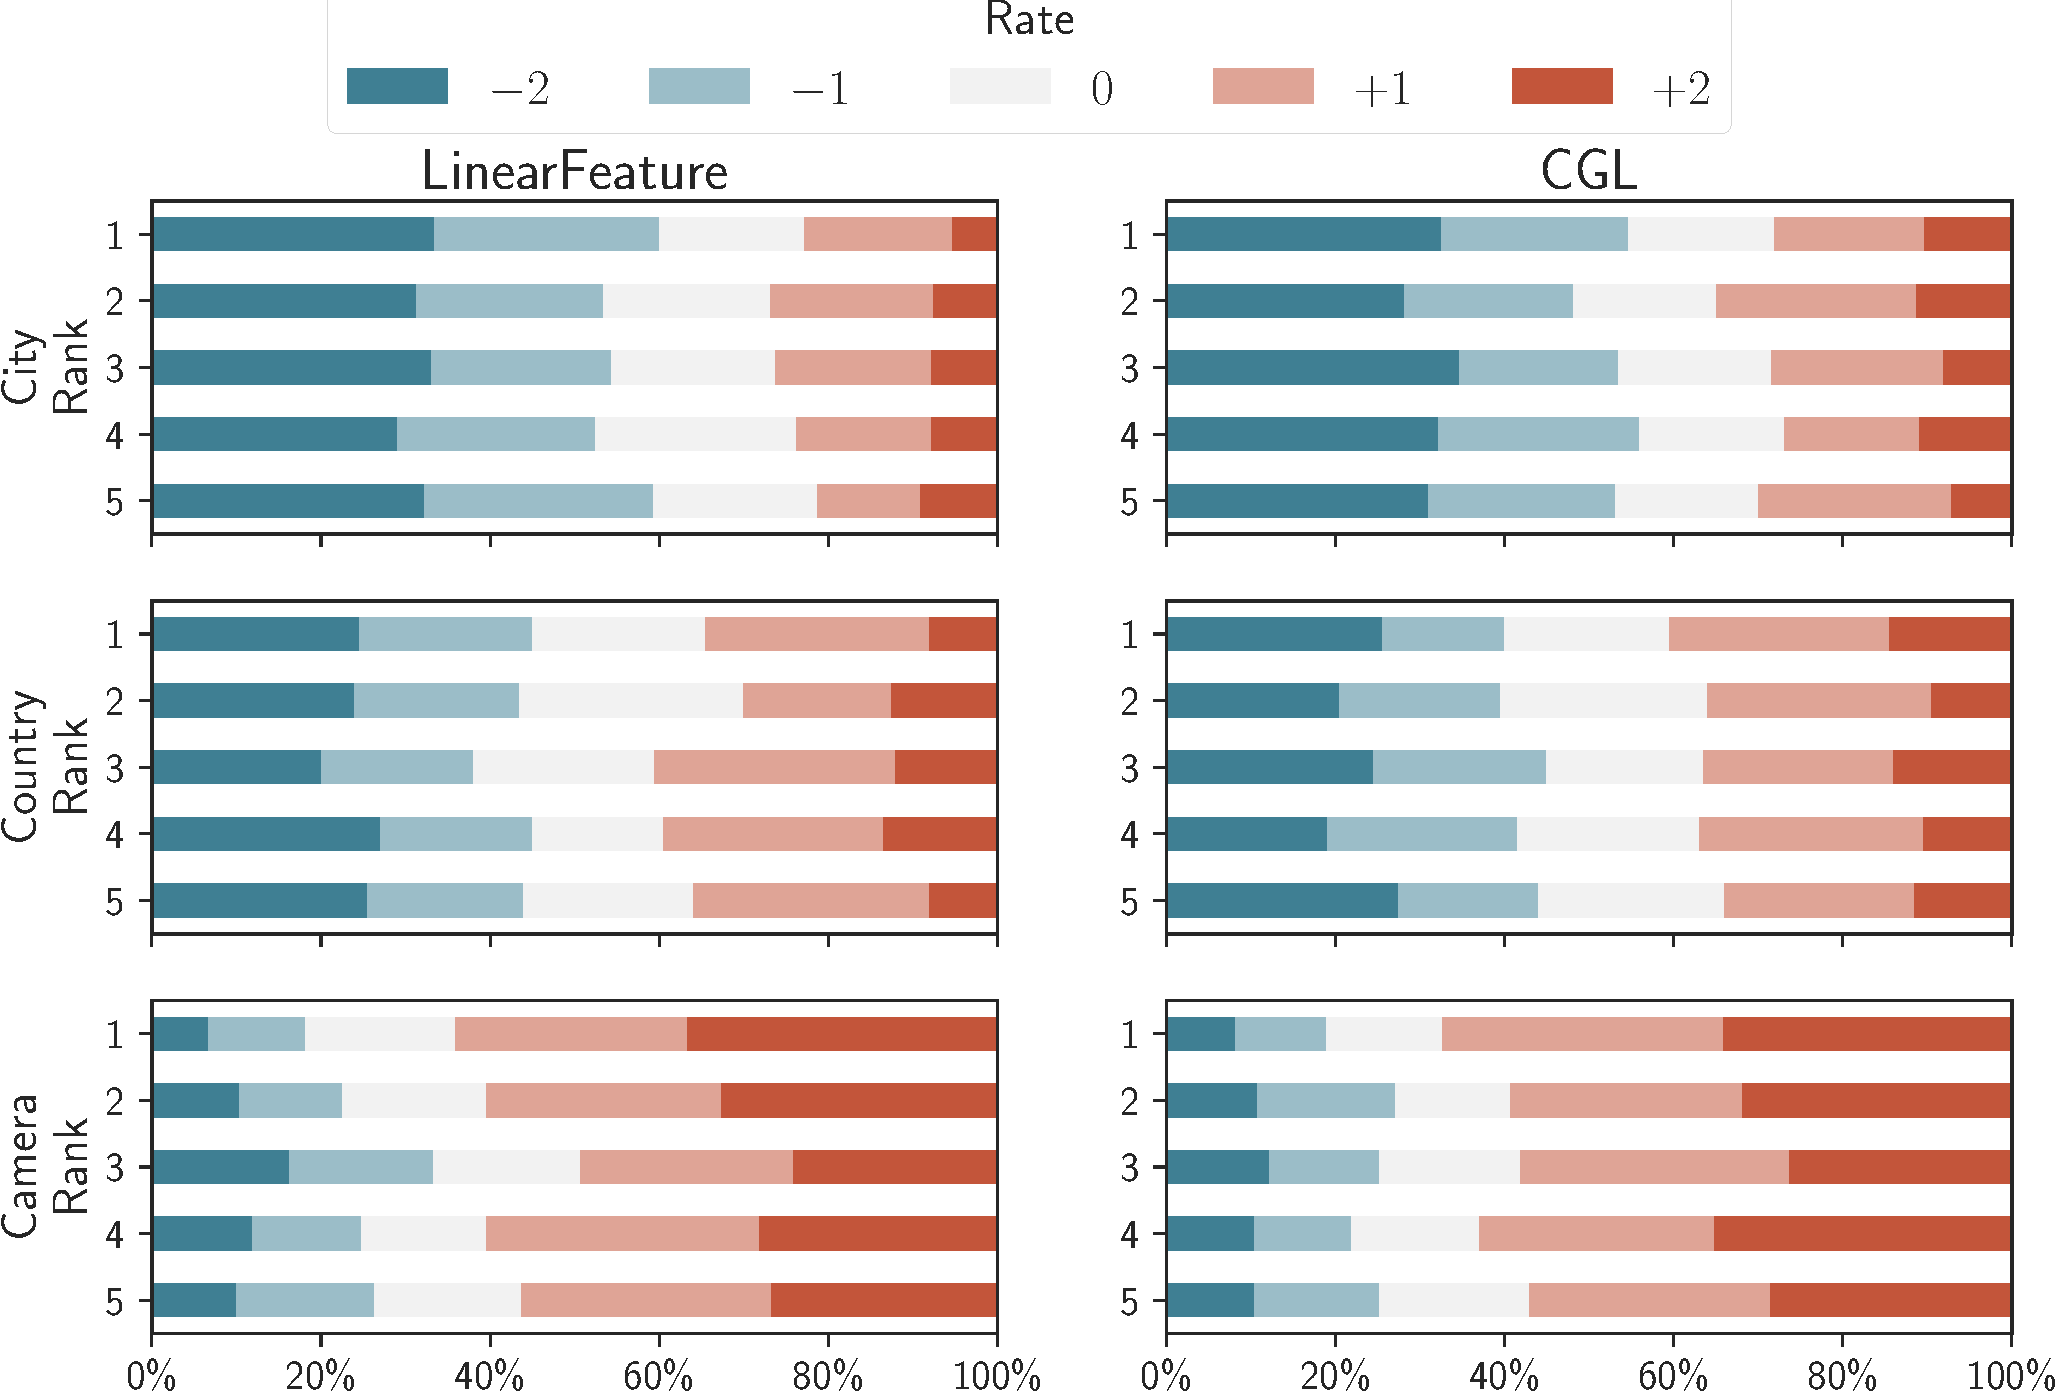
\includegraphics[width=\columnwidth]{images/rates}
    \caption{最も絶対値の高い重みを持つ5つの属性の評価値の分布.}
    \label{fig:weights_evaluation_results}
  \end{center}
\end{figure}

図\ref{fig:weights_evaluation_results}に最も絶対値の高い重みを持つ5つの属性の評価値の分布を示す.
都道府県,国,カメラに対して,文脈誘導型学習の平均評価値はそれぞれ,
$-0.455$,$-0.166$,$+0.581$であり,
LinearFeatureの平均評価値はそれぞれ,$-0.560$,$-0.204$,$+0.516$であった.
これらの評価値は手法の精度と高い相関がある.
文脈誘導型学習はすべてのクラスにおいてLinearFeatureよりも妥当な属性を発見できていたが,全てのクラスにおいてその差はわずかである.
都道府県と国における平均評価値は0以下となっており,各属性の低い説明可能性を示唆している.
これは単に各属性が順序基準と相関があったものの,
順序基準に変化をもたらす要因として評価されなかったためではないかと考えている.
文脈誘導型学習はベースラインよりも精度が高いモデルを学習できたものの,
与えられた順序基準に対して高い説明可能性を持った属性を発見するのは未だ挑戦的な課題であると言える.

\begin{table}[t]
\centering
\caption{文脈誘導型学習によって学習された線形関数の例.最も絶対値の高い重みを持つ3つの属性のみを示している.
}
\scalebox{0.725}{
\begin{tabular}{l p{1em} l c c l c l c l }
\toprule
クラス&&\multicolumn{8}{c}{学習された線型モデル}\\
\midrule
都道府県&&魅力度&$=$&$+0.035$&女性の平均寿命&$-0.032$&交通事故死者数&$-0.031$&人口/世帯数\\
都道府県&&貯蓄額&$=$&$-0.174$&最高気温&$+0.160$&健康寿命&$+0.148$&旅館数\\
国&&評判&$=$&$+0.058$&幸福度 &$-0.057$&難民申請数& $-0.045$&自殺者数\\
国&&平和&=&$+0.170$&穀物収穫量&$+0.166$&GDP成長率&$-0.126$&自殺者数\\
カメラ&&操作性&$=$&$-0.240$&重さ&$-0.213$&高さ&$+ 0.133$&シャッタースピード\\
\bottomrule
\end{tabular}
}
\label{tb:learnt_models}
\end{table}

最後に,文脈誘導型学習によって学習された線形関数の例を表\ref{tb:learnt_models}に示す.
多くの属性はエンティティ順序を説明可能で影響を与えているように見える.
一方,いくつかの属性はエンティティ順序を説明するために適切でないように見えるが(例えば,``魅力度''に対する``世帯当たりの人口''や``貯蓄額''に対する``最高気温''),
データセット中ではエンティティ順序と高い相関を示している.
これらは主観的評価では妥当でないと判断されたものの,
予測においては大きく貢献している属性の例である.


\chapter{結論}
\label{sq:Conclusions}

本論文では,部分的に観測された順序を訓練データ,エンティティの数値属性を特徴として線形関数を学習することで,エンティティの順序を学習する問題に取り組んだ.
この問題では,訓練データの数が非常に少ないため,
我々は文脈誘導型学習という機械学習手法を提案した.
文脈誘導型学習は,ラベル付けされたデータだけでなく,
各特徴の重みを学習するためにラベル基準と特徴に関する文脈を利用する.
実験では文脈誘導型学習によって既存のランキング学習手法を上回る高い精度が得られることが明らかとなった.

今後の課題としては,文脈誘導型学習の理論的解析,
文脈誘導型学習の他の問題への応用(マルチラベル学習やゼロショット学習),
より良い文脈モデルの検討,大規模データに対応するため効率化などを挙げる.
%
%TC:ignore
\backmatter
\pagenumbering{roman}
%
% 謝辞
\chapter*{謝辞}
\addcontentsline{toc}{chapter}{謝辞}

本研究に取り組むにあたり,多大なるご指導を賜りました京都大学大学院情報学研究科の吉川正俊教授,
馬強教授、浅野泰仁特定准教授,アダムヤトフト特定准教授,
山本岳洋助教に深く御礼を申し上げます. 
また, 日頃より様々なご協力をいただきました吉川・馬研究室の皆様に感謝の意を申し上げます.
%
\cleardoublepage
\bibliographystyle{sist02}
% 参考文献
\bibliography{bibliography}
%
%TC:endignore
%
% 付録
% \appendix
% \chapter{付録}
\def\thesection{\Alph{section}}

\section{付録1}

これは付録の例です.基本的には利用しなくて良い.

\section{付録2}

これは付録の例です.基本的には利用しなくて良い.

\subsection{付録2.1}

これは付録の例です.基本的には利用しなくて良い.

\end{document}